
The results previously shown were obtained without considering hardware noise. We observed that VAns was able to better exploit the quantum resources at hand (\textit{i.e.} attain a lower cost-function value) as compared to its fix-structure counterpart (\textit{e.g.} HEA).

\begin{figure}[h!]
\centering
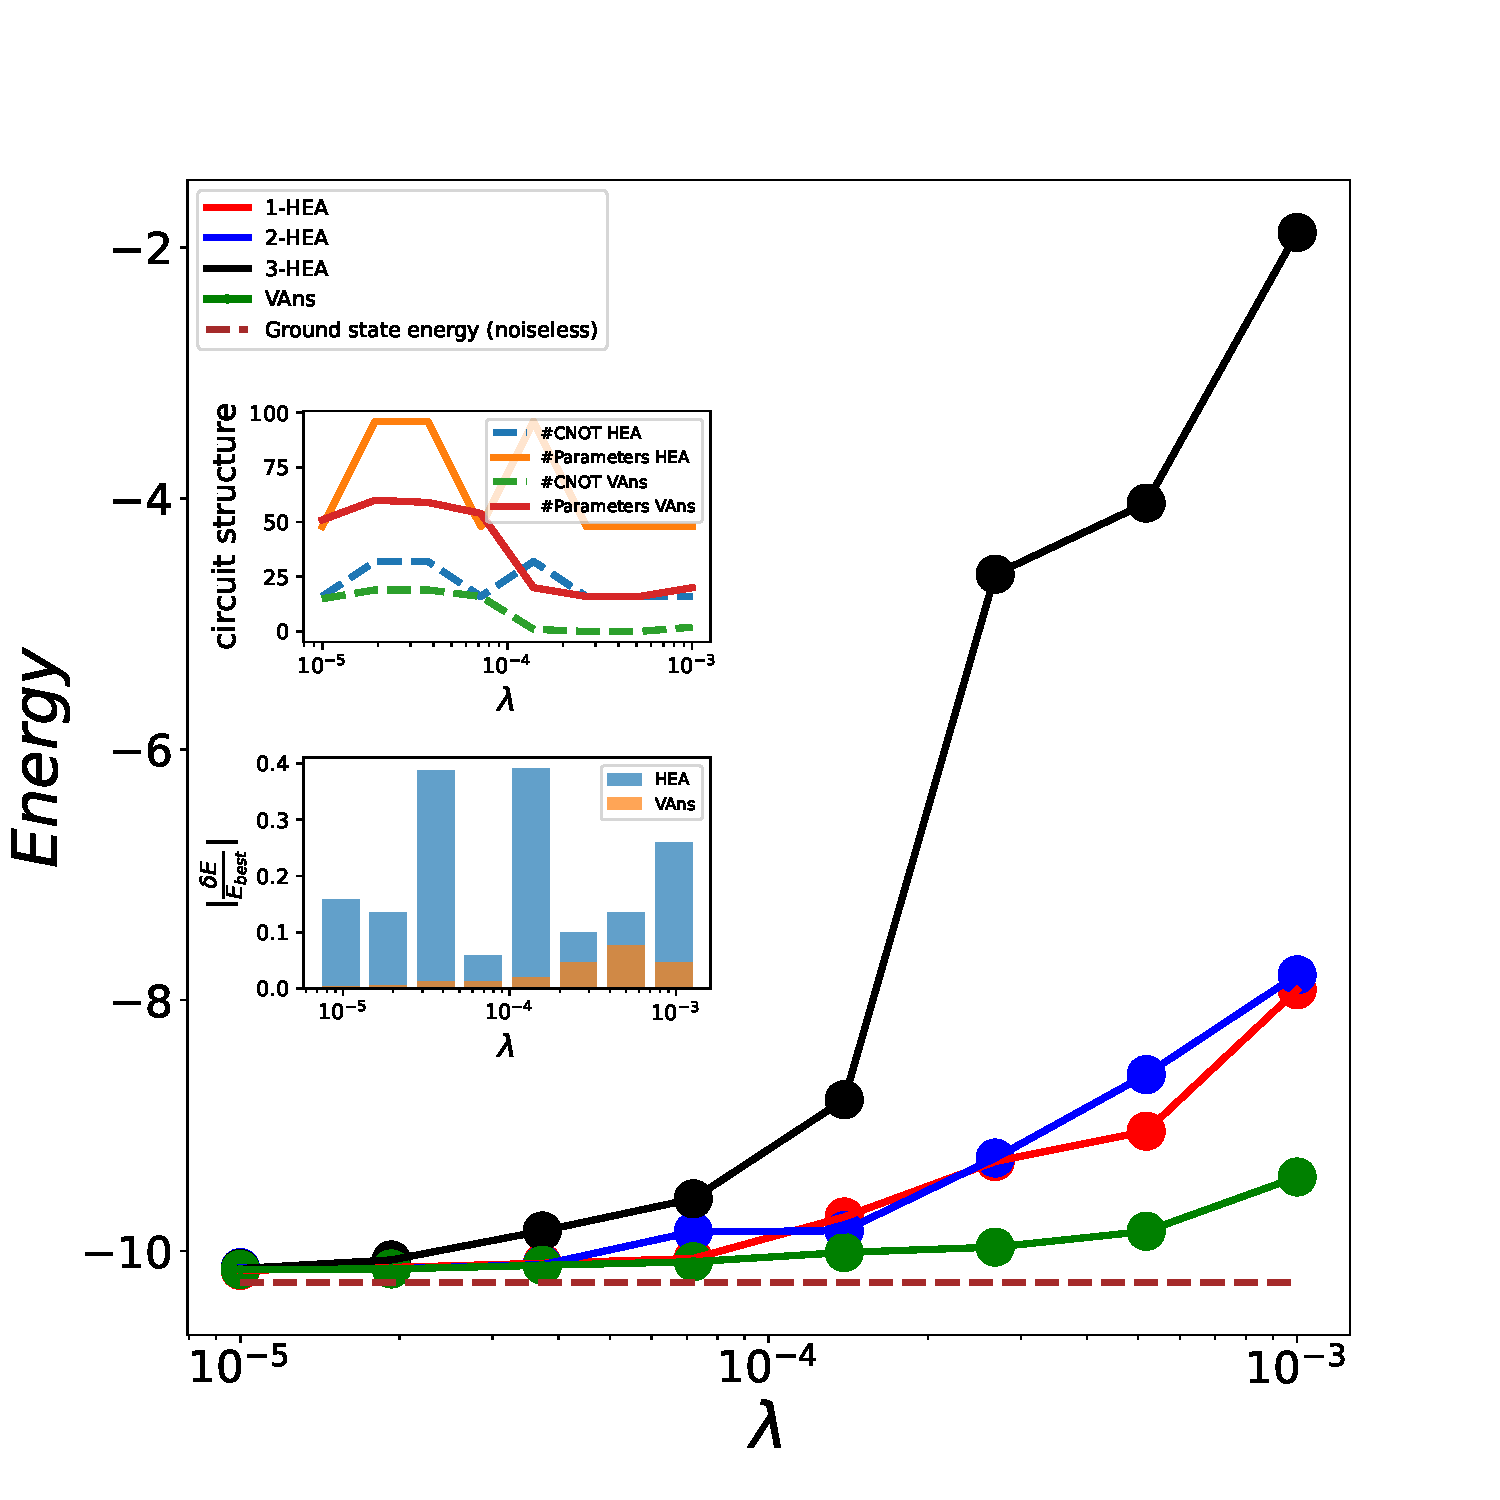
\includegraphics[width=.9\textwidth]{Figures/VANS/Fig13.pdf}
\caption{Results of using VAns for VQE under the $\lambda$-model. Here we consider the TFIM for 8 qubits, with $g=J=1$. The results are obtained after repeating 50 iterations of optimizations with VAns and HEA respectively. We observe that VAns discovers much more efficient quantum circuits as compared to HEA. As shown in the upper inset, VAns automatically adjusts the circuit layout according to the noise strength at hand, a feature that fix-structure ansatzes lack. In the lower inset we show the relative errors (\textit{e.g.} standard deviation over optimal cost found) for both ansatzes, across the 50 iterations; we observe that VAns is more precise in reaching a minimum as compared to HEA. We note that in this experiment we have initialized VAns to a 1-HEA, which is in turn inconvenient for a sufficiently high value of $\lambda$. Yet, VAns learns how to adapt the ansatz (in this case, finding a separable one) so to reach the lowest cost value. In all cases VAns termination criteria was set to a maximum number of 30 iterations.}
\label{fig:Fig13}
\end{figure}

We now consider the case where noisy channels are present in the quantum circuit, an unavoidable situation in current experimental setups, with noise essentially forbidding large-depth quantum circuits to preserve quantum coherence. In the context of QML, the overall effect of noise is that of degrading the cost-function value and, if its strength is sufficiently high, then short-depth circuits turn to be favoured even at the cost of expressibility. For instance, increasing the number of layers in HEA ansatz might not reduce the cost function and even increase it, since noise accumulates due to the presence of gates.

There are several sources of noise in quantum computers. For instance, experimental implementation of a quantum gate takes a finite amount of time, which in turn depends on the physical qubit at hand, the latter subjected to thermal relaxation errors. Relaxation and dephasing errors depend, in general, on each particular qubit (i.e. \textit{the qubit label}). The overall effect of the gate implementation is often modeled by a depolarizing quantum channel, followed by phase flips and amplitude damping channels, whose strength depends on the aforementioned parameters (gate implementation time, qubit label), gate type and environment temperature. For instance, an entangling gate such as a CNOT injects considerably more noise to the circuit than a single-qubit rotation. Moreover, state initialization and readout errors should be taken into account. We refer the reader to find further details on noise modeling in Ref.~\cite{Georgopoulos2021Modeling}. We also note that additional sources of noise should ultimately be considered, such as idle noise and cross-talk effects~\cite{larose2022error, Prakash2020Software}. Because the complexity of noise modelling in NISQ devices is particularly high, we here propose a sufficiently simple model that yet captures the essential noise sources.

\textbf{The $\lambda$-model}. While a noise-model is ultimately linked to the specific quantum hardware at hand and depends on several factors, we propose a unifying and simplified one that depends on a single parameter. The main motivation behind this is that of benchmarking the performance of different ansatzes in the presence of noise. In more complex scenarios, one should consider specific process matrices obtained from \textit{e.g.} process tomography~\cite{Obrien2004Quantum,Zhou2014Process}, which would here obscure the benchmark and also bias it towards specific quantum hardware. In particular, our model is inspired by Refs~\cite{Blank2020Quantum, Georgopoulos2021Modeling}, which in turn are implemented in the \texttt{aer noise simulator} of IBM, and consists of the following models. State preparation and measurement errors are modeled via bit flip channels acting on each qubit, with strength $\lambda \; 10^{-2}$, happening before the circuit $U(\kvec, \thv)$ and measurements respectively. Noise due to gate implementation is modeled as a depolarizing channel, followed by a phase flip and amplitude damping channels acting on the target qubit right after the gate. In principle, the strength of the channel should depend on the specific qubit, and gate type, but in order to keep the model simple enough we have assumed no noise dependence on the qubit label. Moreover, a two-qubit gate is considerably more noisy than a single-qubit one, which in the $\lambda$-model is reflected by the fact that noise strengths are an order of magnitude higher, in the depolarizing channel, than in single-qubit gates, the latter being $\lambda \; 10^{-5}$. Finally, the strengths of the phase flip and amplitude damping channels are set to $\lambda \; 10^{-3}$. We note that, while not considered here, different situations can easily be incorporated such as qubit connectivity constraints, or differences in qubits' quality (some qubits might be noisier than others). In such cases, we expect VAns to find circuits which automatically balance the trade-offs at hand, \textit{i.e.} minimize the number of gates acting on such noisier qubits.

With this model at hand, we have explored the region of $\lambda$ in which the action of the noise becomes \textit{interesting}. The results of running VAns under the $\lambda$-model for ground state preparation (VQE) of TFIM 8-qubit system are shown in Fig.~\ref{fig:Fig13}. Here, the noise strength is sufficiently high so to affect the ground-state energy (which can otherwise be attained by either VAns or a 3-HEA). We thus sweep the value of $\lambda$ by two orders of magnitude, and compare the results that VAns reaches with those of HEA (varying the number of layers of the latter). We see that for a sufficiently high noise strength, increasing the number of gates (e.g. the number of layers in HEA) eventually degrades the cost-function value, as opposed to the noise-less scenario. On the contrary, we observe that even if the noise-strenght is sufficiently high, VAns considerably outperforms HEA by automatically adjusting the depth of the circuit to the noise-strength at hand. Thus, if the noise is large, shallow circuits are found, whereas if the noise-strength is low, deeper circuits are allowed to be explored, since the penalty of adding new gates is smaller. In general, we observe that VAns is capable of finding the best possible circuit under given conditions, which is something that HEA simply can not accomplish.

\afterpage{\clearpage}
